\documentclass[hidelinks, a4paper,twoside]{punch_report}
\usepackage{array, boldline, makecell, booktabs}
\newcommand\btrule[1]{\specialrule{#1}{0pt}{0pt}}
\usepackage{colortbl}
\usepackage{multicol,caption}               % three-column layout
\usepackage[font={footnotesize}]{caption}
\usepackage{xcolor}
\usepackage{amsmath}
% \usepackage{ae}
\usepackage{geometry}
\usepackage{multirow}
\usepackage{siunitx}
\usepackage[title]{appendix}
\usepackage{longtable} 
\usepackage{hyperref}
\usepackage{flafter}
\usepackage{afterpage}
\usepackage{varioref}
% \usepackage[utf8]{inputenc}
\usepackage{graphicx}
\usepackage{setspace}
\setstretch{2}
\usepackage[many]{tcolorbox}
\usepackage{float}
\usepackage{xcolor}
\hypersetup{
    colorlinks,
    linkcolor={blue!70!black},
    citecolor={blue!50!black},
    urlcolor={blue!80!black}
    }
\usepackage{xepersian-multiplechoice}
\usepackage{xepersian}
\settextfont[Scale=1.4]{XB Niloofar}
% \setlatintextfont[Scale=1.3]{Times New Roman}
%\usepackage{draftwatermark}
%\SetWatermarkText{Draft}
%\SetWatermarkScale{1}

% \newenvironment{Figure}
%   {\par\medskip\noindent\minipage{\linewidth}}
%   {\endminipage\par\medskip}

  
% \title{دفترچه محاسبات سازه}
% \newcommand{\punch}{نرم افزار برش پانچ}
% \newcommand{\address}{شهرک شکوهیه فاز 2 خ بابایی خ تهرانی مقدم نبش فرعی 5}
% \author{ابراهیم رعیت رکن آبادی}
% % \date{}
% \today{}

%\vspace{3cm}\textbf{NOTE: This preliminary  report is simply deemed suitable for the purpose of pre-dimensioning the structures addressed and obtaining the loads transmitted by them upon the foundation. The equipment modelling doesn't reflect its final geometric characteristics.}}
% \renewcommand{\revision}{1.0}

\begin{document}
% \begin{center}
%   بنام خدا \newline
%   \maketitle
%   \vspace{10cm}
%   مالک: شرکت سلامت گستران پردیس پارت
%   \newline
%   پلاک ثبتی:
% \end{center}


% \newpage
% \renewcommand{\abstractname}{Executive Summary}.
% \maxdeadcycles=200

% %\maketitle
% \tableofcontents
% \listoftables
% \listoffigures
% \newpage
\pagenumbering{Roman}    % a, b, c, ...
\thispagestyle{empty}
% نحوه درج کردن لوگوی دانشگاه
\begin{figure*}[!h]
\centerline{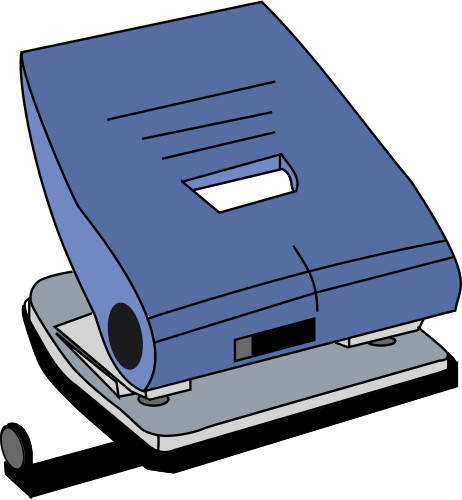
\includegraphics[width=4cm]{logo}}
%\caption{}
\end{figure*}
\begin{center}
%دستوری برای کم کردن فاصله بین لوگو و خط پایین آن
\vspace{-.8cm}

% {\large پژوهشگاه بین المللی زلزله شناسی و مهندسی زلزله}
%دستوری برای تعیین فاصله بین دو خط


\\[1cm]
بنام خدا
\\[1cm]
راهنمای کاربری
\\[.8cm]
% {\nastaliq
\begin{Huge}
نرم افزار 
\lr{CivilTools}
\end{Huge}

\\[.5cm]
\begin{latin}
    \textbf{Ver. 5.0}
\end{latin}



\begin{figure}[ht]
    \centering
        
\includegraphics[width=\linewidth]{figures/civiltools}
        % \caption{DL, units:[m,kN]}
        % \label{dl-unitsmkn}
\end{figure}

\\[2.5cm]{ توسعه دهنده:}
\\[.3cm]
\textbf{{\large  \developer}}

% \\[2cm]{کارفرما}
% \\[.3cm]
% \textbf{{\large \karfarma}}
% \\ \textit{\address}

\\[1.cm]
\today
\end{center}
%\maketitle
%دستوری برای رفتن به صفحه جدید
\newpage
\thispagestyle{empty}
% \pagenumbering{Roman}   % i, ii, iii, iv, ...
\setcounter{page}{1}
\tableofcontents
% \listoffigures
% \listoftables
\newpage

\pagenumbering{arabic}
\section*{مقدمه}

محاسبه برش پانچ در نرم افزار سیف به صورت صحیح  همیشه یکی از دغدغه های مهندسین عمران بوده است. خود من همیشه برای محاسبه پانچ با مشکل روبرو می شدم. بعد از آشنایی با نرم افزار 
\lr{FreeCAD}
و بررسی قابلیت های آن تصمیم گرفتم نرم افزار برش پانچ را با استفاده از ابزارهای قدرتمند این نرم افزار ایجاد کنم. مهمترین مشکل این کار، تشخیص درست صفحات پانچ و موقعیت ستون بود که به لطف خدا  الگوریتم
بسیار دقیقی برای این کار نوشتم که در تمامی موارد صفحات و موقعیت ستون ها را به درستی تشخیص میدهد.


نرم افزار حاضر، نرم افزاری کدباز برای محاسبه برش پانچ فنداسیون با استفاده از خروجی نرم افزار سیف می باشد. این نرم افزار با تلاش های شبانه روزی تهیه شده است و در توسعه آن سعی شده است که ضمن داشتن رابط کاربری آسان، 
نتایج نرم افزار از دقت بسیار بالایی برخوردار باشد. امیدوارم که  برای مهندسین عزیز مفید باشد.



کانال تلگرام: \lr{@civiltools} \newline
آی دی تلگرام: \lr{@roknabadi}

\newpage
% \begin{twocolumn}
\section{ساخت فایل خروجی اکسل در سیف\label{sec:prepare-safe}}
مراحلی که در زیر آمده است برای آماده سازی فایل نرم افزار برش پانچ کفایت میکند. بنابراین نیاز به انجام کار اضافی نیست. مثلا نیاز به تخصیص سختی خاک، المانهای ستون
\lr{(Stiff)}
و ... نمی باشد.


\subsection{ترسیم هندسه پی}
در این مرحله فقط هندسه پی مطابق شکل 
\ref{geometry}
ترسیم می شود. سعی کنید در این مرحله تمیزکاری زیادی نکنید. منظورم این هست که 
\textbf{هم پوشانی}
 نوارهای فنداسیون چه در سیف و چه در نرم افزار برش پانچ مشکلی ایجاد نمیکند،
بنابراین سعی نکنید که لبه های نوارها را بهم بچسبانید، بلکه اجازه دهید مقداری هم پوشانی در نوارها ایجاد شود.
برای ترسیم پی های نواری میتوانید از 
\textbf{بازشو}
 هم استفاده کنید و نرم افزار برش پانچ با ترسیم بازشو مشکلی ندارد و محاسبات پانچ به درستی انجام میگیرد.

\begin{figure}[H]
    \centering
    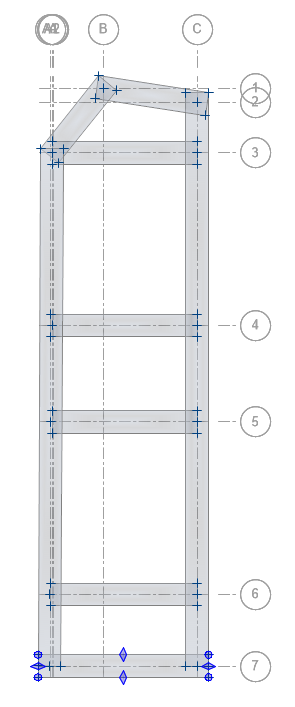
\includegraphics[scale=.6]{figures/geometry2}
    \caption{ترسیم هندسه پی در سیف}
    \label{geometry}
\end{figure}


\subsection{اختصاص مقطع به پی}
در این مرحله از منوی 
$Assign \rightarrow Slab Data \rightarrow Properties$
به هندسه ترسیم شده مقطع مناسب را اختصاص دهید (شکل 
\ref{assign}):

\begin{figure}[H]
    \centering
    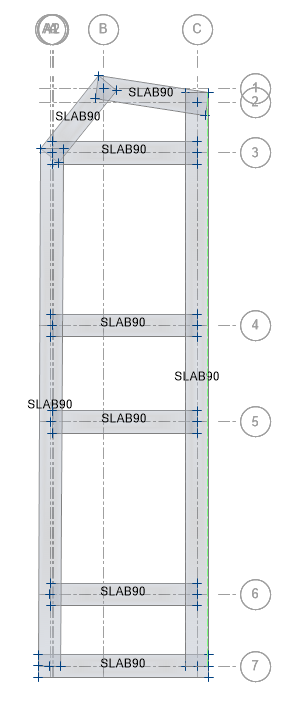
\includegraphics[scale=.6]{figures/assign}
    \caption{اختصاص مقطع به پی}
    \label{assign}
\end{figure}


\subsection{خروجی به اکسل}
مطابق شکل 
\ref{excel}
از منوی 
$File \rightarrow Export Model \rightarrow Excel $
خروجی به اکسل را انتخاب کنید. مطابق شکل 
\ref{excel2}
تیک بخش
\lr{MODEL DEFINITION}
را بزنید و 
در قسمت 
\lr{Select Load Patterns}
تمامی الگوی بارها را انتخاب و واحد خروجی را 
$KN, mm, C$
برگزینید. فایل را در محل دلخواه ذخیره کنید.

\begin{figure}[H]
    \centering
    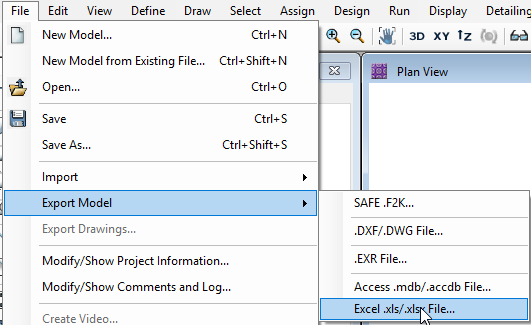
\includegraphics[width=.7\linewidth]{figures/excel}
    \caption{خروجی به اکسل}
    \label{excel}
\end{figure}

\begin{figure}[H]
    \centering
    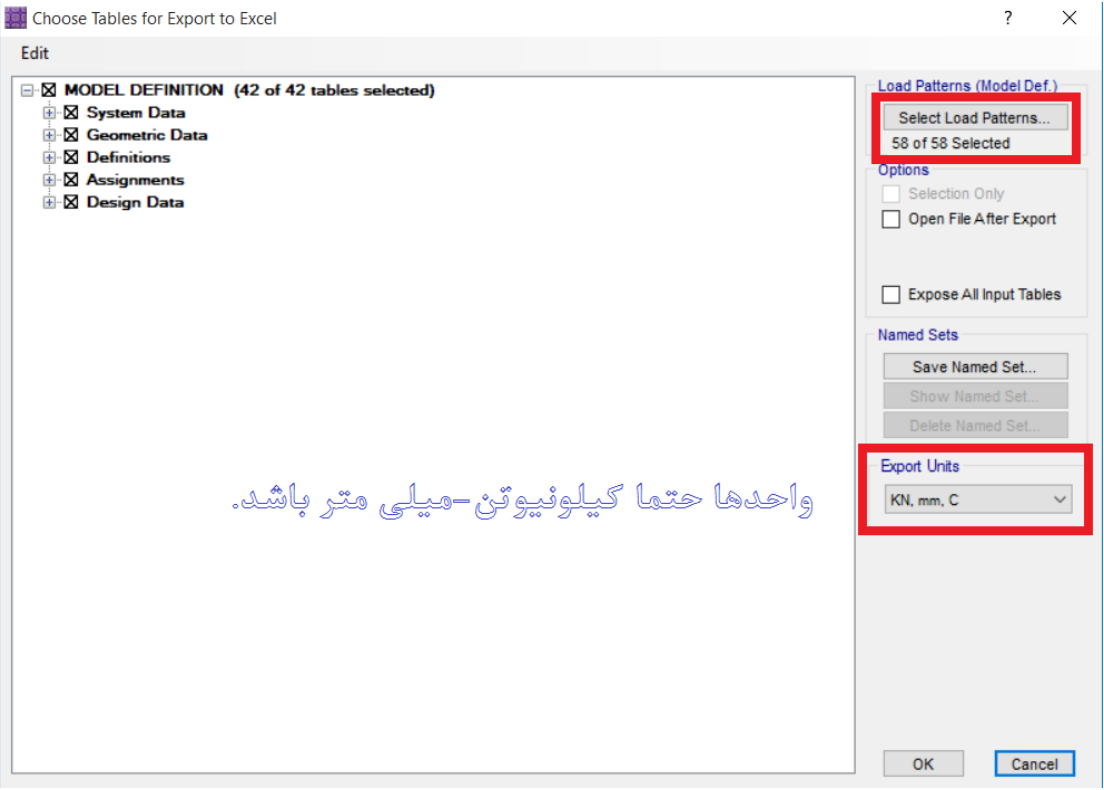
\includegraphics[width=.7\linewidth]{figures/excel2}
    \caption{تنظیم پارامترهای خروجی فایل اکسل}
    \label{excel2}
\end{figure}
\section{محاسبه برش پانچ در \lr{FreeCAD}}

\subsection{بارگذاری ورک بنچ \lr{Civil}\label{sec:loadingcivil}}
بعد از باز کردن نرم افزار 
\lr{FreeCAD}
، مطابق شکل
\ref{fig:civil-workbench}
با کلیک روی منوی کرکره ای ورک بنچ ها، از لیست موجود 
\lr{Civil}
را انتخاب کنید. با این کار منو و آیکون های نرم افزار برش پانچ ظاهر میشوند. برای اینکه هر دفعه پس از بازکردن نرم افزار نیاز به این کار نداشته باشید به قسمت
\ref{faq}
 مراجعه کنید.

\begin{figure}[H]
    \centering
    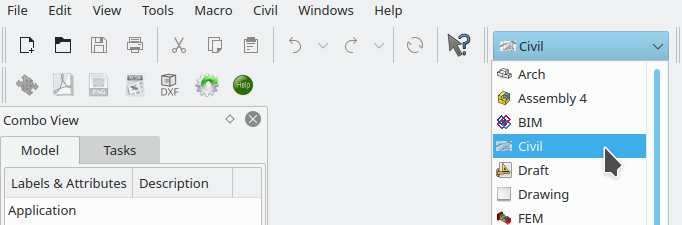
\includegraphics[width=\linewidth]{figures/civil}
    \caption{بارگذاری ورک بنچ \lr{Civil}}
    \label{fig:civil-workbench}
\end{figure}
\subsection{بازکردن فایل اکسل}
برای فراخوانی فایل اکسلی که در بخش 
\ref{sec:prepare-safe}
ساختیم، کافیست که آنرا مثل یک فایل اکسل در نرم افزار باز کنید. یعنی از منوی
$File \rightarrow Open$
این کار را انجام دهید. در این مرحله حتی نیاز به فراخوانی ورک بنچ 
\lr{Civil}
نمی باشد. بعد از چند لحظه فنداسیون داخل نرم افزار بارگذاری شده و محاسبات پانچ برای تمامی ستونها صورت میگیرد.

\subsection{ذخیره پروژه}
در ورژن جدید میتوانید به سادگی مثل سایر نرم افزارها پروژه را ذخیره و باز کنید. بعد از بازکردن پروژه های ذخیره شده میتوانید ویرایش های لازم را انجام دهید. این قابلیت در 
ورژن های قبلی نرم افزار موجود نبود.
\section{تغییر مشخصات پانچ ها}

نرم افزار برش پانچ به گونه ای نوشته شده است که تقریبا در تمامی موارد پانچ ستونها را بدرستی تشخیص داده و نسبت آنها را محاسبه میکند. با این حال برای اینکه کاربر بتواند کنترل بیشتری روی 
پارامترهای مختلف محاسبه پانچ داشته باشد، ارتفاع فنداسیون، مقاومت بتن فنداسیون، ابعاد ستونها و موقعیت ستونها در نرم افزار قابل ویرایش هستند.
با تغییر هر یک از پارامترها پانچ تمامی ستونها مجددا محاسبه میشود. ممکن است ستونی که به صورت کنار شناخته شده است با افزایش ضخامت فنداسیون به صورت گوشه شناخته شود و در نتیجه 
نسبت تنش پانچ آن افزایش یابد!

\subsection{تغییر مشخصات فنداسیون}
ضخامت، کاور و مقاومت بتن فنداسیون را میتوان در نرم افزار تغییر داد. برای این کار کافیست که در محیط سه بعدی نرم افزار روی فنداسیون کلیک کنید. با این کار در جدول سمت چپ با نام
\lr{Combo View}
مشخصات فنداسیون به نمایش در می آید (شکل 
\ref{fig:comboview}
). اگر مشخصات قابل رویت نیست به بخش سوالات متداول مراجعه کنید. 
% \ref{faq:dataview}

\begin{figure}[H]
    \centering
    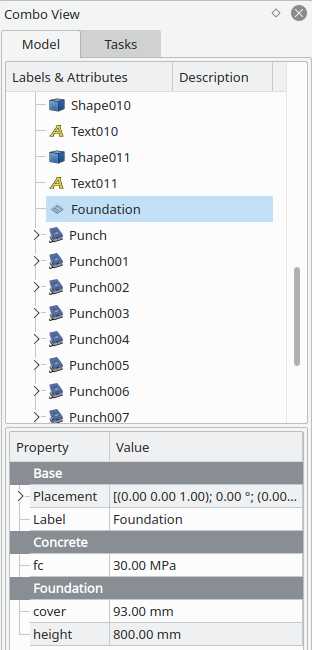
\includegraphics{figures/comboview}
    \caption{تغییر مشخصات فنداسیون}
    \label{fig:comboview}
\end{figure}

\subsection{تغییر مشخصات ستونها}
ابعاد و موقعیت ستونها را میتوان تغییر داد. برای این کار در محیط سه بعدی نرم افزار روی هر کدام از ستونها که قصد تغییر مشخصات آنرا دارید کلیک کنید.
با این کار در جدول سمت چپ مشخصات ستون ظاهر میشود که میتوان ابعاد ستون،
$b_x, b_y$
و موقعیت ستون، 
\lr{Location}
را تغییر داد. برای تغییر ابعاد ستون کافیست که عدد مورد نظر خود را برای ابعاد ستون وارد کنید.
برای تغییر موقعیت ستون ابتدا باید پارامتر 
\lr{user modified}
را از حالت 
\lr{false}
به 
\lr{true}
تغییر دهید و سپس موقعیت جدید ستون را با پارامتر
\lr{Location}
تغییر دهید. دقت کنید که فقط میتوان از پانچ وسط به کنار و گوشه 
و از پانچ کنار به گوشه تغییر موقعیت داد. چون باید صفحات مناسب پانچ برای تشخیص وجود داشته باشد.
یعنی نرم افزار با تغییر موقعیت ستون، یک یا دو صفحه پانچ را حذف میکند، ولی نمیتوان صفحه ای که وجود ندارد را به آن اضافه نمود!

\begin{itemize}
    \item نکته: بجای اینکه ویرایش را جدول کنار نرم افزار انجام دهید میتوانید با دابل کلیک روی اسم هر کدام از پانچ ها در قسمت بالایی جدول
    \lr{Combo View}
    این کار را انجام دهید. پس از دابل کلیک روی نام پانچ مورد نظر، یک پنجره مطابق شکل
    \ref{fig:columnedit}
    باز میشود که میتوانید موقعیت و ابعاد ستون را در آن تغییر دهید. در این پنجره نیز برای تغییر موقعیت ستون تیک مورد نظر را بزنید.
\end{itemize}

\begin{figure}[H]
    \centering
    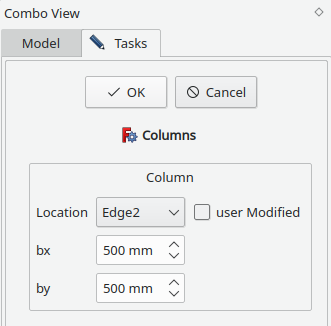
\includegraphics{figures/columnedit}
    \caption{پنجره تغییر مشخصات ستون}
    \label{fig:columnedit}
\end{figure}

\section{ذخیره نتایج خروجی}
برای گرفتن خروجی از نرم افزار، میتوانید از آیکون های مرتبط برای فرمت های مختلف استفاده کنید. در حال حاضر نرم افزار قادر به خروجی نتایج گرافیکی پانچ ها به فرمت عکس، 
پی دی اف و اتوکد می باشد. همچنین محاسبات پانچ برای تمامی ترکیب بارها را میتوان به صورت فایل اکسل ذخیره نمود. اگر آیکن ها وجود ندارند و یا اینکه منوی 
\lr{Civil}
در منوهای نرم افزار موجود نیست باید ابتدا طبق بخش
\ref{sec:loadingcivil}
ورک بنچ را فعال نمایید.

\begin{figure}[H]
    \centering
    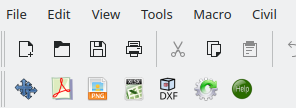
\includegraphics{figures/export}
    \caption{منو و آیکن های خروجی نرم افزار}
\end{figure}
\section{آپدیت نرم افزار}
برای آپدیت به آخرین تغییرات نرم افزار کافیست که روی آیکن شکل چرخ دنده کلیک کنید. برای اولین بار احتمالا حدود ۲-۳ دقیقه برای آپدیت نرم افزار زمان نیاز است.
بعد از اتمام نصب، پوشه 
\lr{Civil}
در محل نصب نرم افزار را پاک کنید. به طور معمول پوشه 
\lr{Civil}
در مسیر زیر قرار دارد:

\begin{center}
    
    \lr{C:\textbackslash Program Files\textbackslash FreeCAD\textbackslash mod}
\end{center}


نرم افزار را مجددا راه اندازی کنید. برای آپدیت های بعدی نیاز به پاک کردن فایل نیست، چون اصلا فایلی وجود ندارد!

\newpage
\section{پرسش های متداول\label{faq}}

در این بخش برخی از سوالات متداول که کاربران میپرسند به مرور زمان اضافه میشود.

\begin{question}{مشخصات فنداسیون یا پانچ برای من نمایش داده نمیشود.}
\true 
اگر با کلیک روی فنداسیون یا هر یک از ستونها در محیط سه بعدی یا قسمت بالایی جدول
\lr{Combo View}
مشخصات فنداسیون یا پانچ ها قابل مشاهده نیستند، در قسمت پایین جدول مطمئن شوید که تب 
\lr{Data}
فعال باشد، مطابق شکل
\ref{fig:dataview}.
\end{question}

\begin{figure}[H]
    \centering
    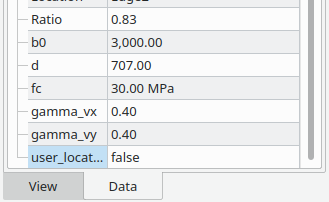
\includegraphics{figures/dataview}
    \caption{تنظیم نمایش مشخصات با انتخاب تب \lr{Data}}
    \label{fig:dataview}
\end{figure}


\begin{question}{چطور هر بار که نرم افزار را باز میکنم به طور خودکار 
    \lr{Civil}
    لود شود؟}
\true 
برای این کار باید از منوی
$Edit \rightarrow Preferences$
پنجره تنظیمات نرم افزار را باز کنید. مطابق شکل
\ref{fig:autoload}
، در تب
\lr{General}
قسمت 
\lr{Start up}
ورک بنچ 
\lr{Civil}
را انتخاب کنید و سپس کلید تایید را بزنید. از این پس بعد از اجرای نرم افزار به طور خودکار ورک بنچ
\lr{Civil}
لود میشود.
\end{question}


\begin{figure}[H]
    \centering
    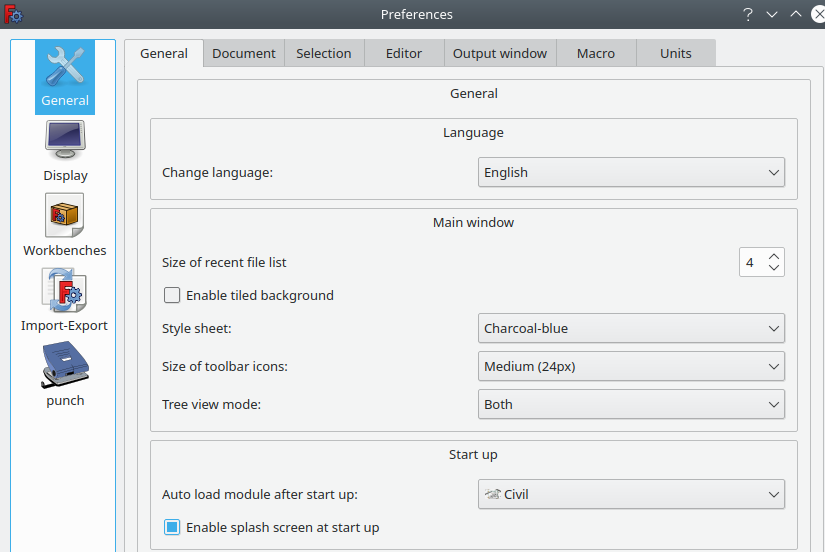
\includegraphics[width=.7\linewidth]{figures/autoload}
    \caption{تنظیم لود شدن خودکار ورک بنچ \lr{Civil} بعد از هر اجرا}
    \label{fig:autoload}
\end{figure}

% \end{twocolumn}
% \section{Combination of loads}
% \input{combinations.tex}
% \input{xc_design_technique.tex}

% \clearpage
% \input{appendix}

% \clearpage
% -----
%------------------------------------------------

%----------------------------------------------------------------------------------------
%	REFERENCE LIST
%----------------------------------------------------------------------------------------
%\phantomsection
%\nocite{OpenSeesManual,FeynmanVolI,Thomson}   % writes also non-cited references
% \nocite{*}
% \bibliography{jubail}  %file .bib 
% \bibliographystyle{plain} %normal style - listed in ABC order and labeled numerically
%\bibliographystyle{unsrt} %same as plain except entries appear in order of citation

% to compile the document run:
%    latex structural_design_report   to create the .aux file
%    bibtex structural_design_report  to get some of the citations and create a .bbl file
%    latex structural_design_report   again so that the cross references between latex file and bibliography
%                               are correct

%----------------------------------------------------------------------------------------

\end{document}
